\documentclass[11pt]{article}
\usepackage[letterpaper,margin=1in]{geometry}
\usepackage[T1]{fontenc}
\usepackage[utf8]{inputenc}
\usepackage{lmodern,microtype}
\usepackage{amsmath,amssymb,booktabs,tabularx,array,graphicx}
\usepackage[dvipsnames]{xcolor}
\usepackage{enumitem,listings}
\usepackage{float}
\usepackage[hidelinks]{hyperref}
\usepackage[section]{placeins}
\newcolumntype{Y}{>{\raggedright\arraybackslash}X}
\setlength{\emergencystretch}{2em}
\setlist{nosep,leftmargin=*}
\lstset{basicstyle=\small\ttfamily,breaklines=true,columns=fullflexible,
 keepspaces=true,showstringspaces=false,frame=single,rulecolor=\color{black!20},
 xleftmargin=4pt,xrightmargin=4pt,aboveskip=9pt,belowskip=9pt}
\newcommand{\takeaway}[1]{\par\smallskip\noindent\textit{What this establishes.} #1\par\medskip}
\newcommand{\pB}{p_{\mathrm B}}
\title{From Confidence to Collective Judgment:\\Task, Experimental Design, and Pilot Notes}
\author{}
\date{18 September 2026}
\begin{document}
\maketitle
\begin{abstract}
We study whether language models change their judgments when the same confidence scores are assigned to different peers. These notes explain the task, the actual prompts, and the completed experiments before describing the remaining research plan. Six instances of one model first predict market demand from separate noisy surveys. We then freeze their initial answers, swap two displayed confidence scores, and ask selected recipients to update. The same comparison is made with and without access to peers' underlying surveys. In two batches, reallocating high confidence toward the high-demand recommendation increased its reported probability by 14.81 and 22.48 percentage points on average when peer surveys were hidden. The corresponding changes with full evidence were small. These are one-step behavioral effects, not evidence of harmful group consensus or validated group prediction. We explain the distinction with a complete worked example, retain unsuccessful earlier experiments in an appendix, and specify the next local-to-group test without assuming the unvalidated dynamics of the original proposal.
\end{abstract}

\section{What is the task, and what is an agent here?}
\label{sec:task}
Imagine that six analysts must forecast whether demand for a new product will be \emph{low} or \emph{high}. Each analyst receives three different survey observations about the same market. The surveys are informative but imperfect. The analysts initially answer separately. Later, an analyst receives reports from the other five and makes a new forecast.

In our experiment an analyst is an \emph{agent}: a separately queried instance of a language model with a neutral identity and a specified input. All six use the same model. We do not train six models, give them expert personas, or assign a supervisor and five subagents. A host program decides which information each request contains. Models do not automatically see one another's responses. For example, the host can send agent 3 its own three surveys plus five saved peer reports, then record its new answer.

Separate requests isolate the visible contexts. They do not imply independent knowledge or uncorrelated mistakes. Because agents receive different surveys, initial disagreement can arise even when each uses its private information correctly. Figure~\ref{fig:task} shows one actual instance.

\begin{figure}[htbp]
\centering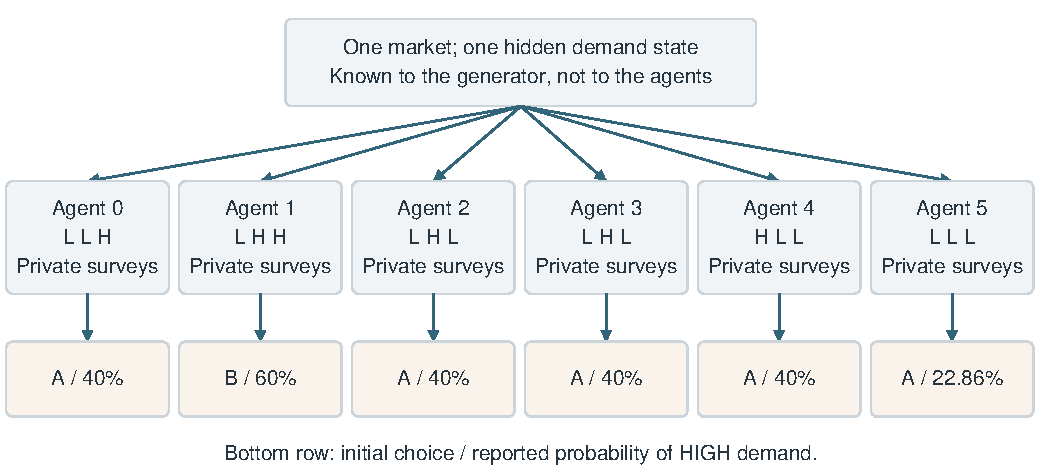
\includegraphics[width=\linewidth]{figures/task.pdf}
\caption{One market and six separate initial responses: replication item \texttt{demand-00}. L/H mean a survey reporting low/high demand. The generator knows the actual state, but it is not sent to agents. The bottom row shows each agent's initial choice and reported probability of \emph{high} demand. Thus A/40\% means ``choose low, with 40\% probability assigned to high.'' Arrows show information flow, not interaction between agents. This diagram has no numerical axes or uncertainty bars.}
\label{fig:task}
\end{figure}

\subsection{The rule supplied to every agent}
The hidden demand state is high or low with prior probability $1/2$ each. A survey reports high with probability $0.6$ when demand is high, and with probability $0.4$ when demand is low. All 18 observations are independent \emph{conditional on the hidden state}. Each agent initially sees exactly three distinct observations. The forecast has three fields:
\begin{itemize}
\item \texttt{answer}: A for low demand, B for high demand;
\item \texttt{p\_B}: the reported probability of high demand, between 0 and 1;
\item \texttt{reason}: one brief sentence.
\end{itemize}
The selection rule is explicit: choose B if $\pB>0.5$, and A otherwise. Each batch contains eight actual high-demand and eight actual low-demand markets before eligibility screening. Apart from this balance, items are not selected for their surveys, initial accuracy, or intervention outcomes.

This is a synthetic forecasting task with a market interpretation. There are no real sales data, human participants, or financial decisions. Its purpose is to make private information and message sharing precise. A result on this task does not establish a law of real markets or human social behavior.

\subsection{Three different percentages}
The following quantities must not be interchanged.
\begin{center}\small
\begin{tabularx}{\linewidth}{@{}p{.23\linewidth}Y@{}}\toprule
Quantity & Meaning \\\midrule
Survey accuracy, 60\% & A property of the observation-generating process, fixed in all conditions. \\
Reported $\pB$, e.g.\ 40\% & The recipient's stated probability that the market has high demand. \\
Displayed confidence, e.g.\ A with 60\% & A number next to a peer's recommendation, defined as that peer's stated probability that its \emph{chosen} state is correct. A/60\% supports low demand; B/60\% supports high demand. \\\bottomrule
\end{tabularx}
\end{center}
Before intervention, an A answer with $\pB=0.4$ implies 60\% confidence in A. During intervention, we overwrite selected displayed confidence values. They no longer necessarily match the sender's private evidence. The recipient's output $\pB$ remains a measured response, not a number supplied by the host.

\takeaway{The task asks agents to reason under partial, noisy information. The experiment changes a cue in peer messages and observes a new forecast. It does not reveal the hidden state to the models.}

\section{Research question and significance}
\label{sec:question}
The immediate question is:
\begin{quote}
With evidence, initial opinions, sender identities, message order, and the set of visible confidence scores held fixed, does changing \emph{who receives the higher score} change the recipient's judgment?
\end{quote}
The second question asks whether access to peers' original evidence changes that response. The longer-term question is whether locally measured responses can predict what an interacting group will do on new items.

These questions matter because a recipient often receives recommendations without being able to inspect all the evidence behind them. A confidence number might then function as a cue about evidence strength. Supplying original evidence might reduce the role of that cue. Establishing when this happens would inform how to evaluate evidence-sharing and confidence-reporting protocols. Whether a particular protocol improves real applications requires additional tests.

The original proposal, \emph{From Confidence to Consensus: Collective Decision Dynamics of LLM Agents}, emphasized assigning high confidence to initially correct versus incorrect members and measuring later group errors. The present task first isolates a more basic contrast: high confidence assigned to an A supporter versus a B supporter. This contrast is defined without consulting the actual demand state. It measures directional influence, rather than assuming the influence is harmful.

Three claims therefore remain separate: (i) scores affect forecasts; (ii) scores improve or impair forecast quality; and (iii) an initial effect changes later group outcomes. A positive result for (i) does not imply (ii) or (iii). Agreement also needs a separate definition: a six-agent consensus means all six choose the same option, regardless of whether that option is correct.

The revision retains the original local-to-group research question and controlled-comparison logic. It removes unvalidated response equations and dynamics claims from the main argument, as well as the old fixed main-study size and budget. The completed experiments, including null and unreplicated findings, remain part of the record.

\takeaway{The current contribution is a controlled test of confidence allocation under different information conditions. Predicting collective reliability remains a research objective.}

\section{One real item, from private evidence to peer reports}
\label{sec:example}
Table~\ref{tab:initial} contains all initial observations and responses for the first eligible item in the replication batch. This item was selected by its saved position, not because it had the largest effect. Its actual demand was low. That state was used for evaluation only.

\begin{table}[htbp]\centering\small
\begin{tabular}{@{}clcc@{}}\toprule
Agent & Private surveys, in order & Initial choice & Reported $\pB$ \\\midrule
0 & low, low, high & A & 0.400000 \\
1 & low, high, high & B & 0.600000 \\
2 & low, high, low & A & 0.400000 \\
3 & low, high, low & A & 0.400000 \\
4 & high, low, low & A & 0.400000 \\
5 & low, low, low & A & 0.228571 \\\bottomrule
\end{tabular}
\caption{Actual initial responses for replication item \texttt{demand-00}. Everyone judges the same market but sees different observations. The final column always refers to \emph{high} demand, including for agents who choose A.}
\label{tab:initial}\end{table}

\subsection{Why agent 3 initially reports 40\%}
Agent 3 sees low, high, low. If demand were high, the probability of that ordered sequence would be $0.4\times0.6\times0.4=0.096$. If demand were low, it would be $0.6\times0.4\times0.6=0.144$. Because the prior probabilities are equal, the conditional probability of high demand is
\begin{equation}
\Pr(H\mid L,H,L)=\frac{0.096}{0.096+0.144}=0.4.
\end{equation}
Two low signals favor low demand, but imperfect surveys leave a substantial possibility of high demand. The model's actual initial response agrees with this calculation. This reference is computed by the researcher for checking; the resulting 0.4 is not inserted as the initial model answer.

\subsection{Why the experimental scores are 60\% and about 77.14\%}
With three surveys, a two-to-one majority yields 60\% probability for the majority state. Three identical surveys yield
\begin{equation}
\frac{0.6^3}{0.6^3+0.4^3}=\frac{27}{35}\simeq0.77142857.
\end{equation}
We use 0.600000 and 0.771429 as the swapped scores. They lie within the task's natural private-evidence range. This choice does not make overwritten scores truthful: agent 4's high, low, low surveys support A at 60\%, even when the host displays 77.1429\% beside its A recommendation.

\subsection{What agent 3 sees when scores are exchanged}
Agents 4 and 1 are the selected A and B senders. Agents 3 and 2 are the recipients. Table~\ref{tab:swap} follows the actual order of reports shown to agent 3. Only the two indicated numbers move.

\begin{table}[htbp]\centering\small
\begin{tabular}{@{}cccc@{}}\toprule
Peer & Frozen recommendation & A-high input & B-high input \\\midrule
5 & A & 0.7714285714 & 0.7714285714 \\
4 & A & \textbf{0.771429} & \textbf{0.600000} \\
2 & A & 0.600000 & 0.600000 \\
1 & B & \textbf{0.600000} & \textbf{0.771429} \\
0 & A & 0.600000 & 0.600000 \\\bottomrule
\end{tabular}
\caption{Displayed confidence in the peer's \emph{chosen} answer. Both inputs contain four A recommendations, one B recommendation, and exactly the same multiset of scores. A-high refers to the selected A sender, not to every A supporter. Agent 3's own surveys and saved forecast are unchanged.}
\label{tab:swap}\end{table}

The recipient sees both swapped senders and is not one of them. This detail matters: if the recipient's own score were exchanged, it would not appear in its inbox, and the visible score collection could change. The local design avoids that confound. Peer 5 keeps its naturally higher score in both inputs.

\takeaway{The comparison does not alter the vote counts, average visible score, evidence, or sender identities. It changes the association between displayed confidence and the A/B recommendation.}

\section{The experimental design, step by step}
\label{sec:design}
\subsection{Two information conditions crossed with the score swap}
In \emph{full evidence}, the recipient sees its own three surveys and all 15 peer surveys, together with peer recommendations and displayed scores. In \emph{advice only}, the recipient retains its own surveys but sees only peers' recommendations and scores. Each update also contains the recipient's genuine initial answer and initial $\pB$. Initial peer reasons and separate peer probabilities are not forwarded.

\begin{figure}[htbp]\centering
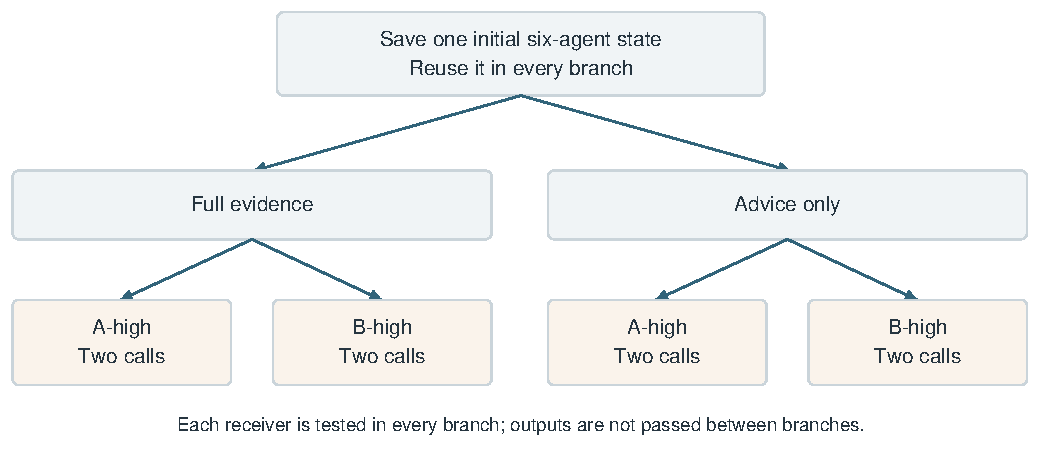
\includegraphics[width=\linewidth]{figures/design.pdf}
\caption{The four main inputs for each recipient. Within either information condition, B-high minus A-high isolates the local score-allocation contrast. Comparing those two contrasts tests whether evidence visibility changes the effect. All requests restart from the same initial state. The diagram omits the equal-pair and hidden-score controls and has no numerical axes.}
\label{fig:design}\end{figure}

Holding an information condition fixed, the two main inputs differ only in the swapped \texttt{confidence} values. Holding a score assignment fixed, full evidence differs from advice only only by the five peer \texttt{surveys} fields. The number of observations per sender, the observation model, and the recipient's own information are known in both conditions.

\subsection{What is run for each item}
\begin{enumerate}
\item Generate one market and 18 surveys, and obtain six real initial responses.
\item If all six responses are valid and include both A and B, randomly select one sender from each camp using the prespecified seed. Select two recipients from the other four agents.
\item Save this initial state once. Construct all updates from it, preserving identities and the randomized inbox order within matched comparisons.
\item For each recipient, test both information conditions and four score conditions: A-high, B-high, equal-pair, and hidden. Call each input twice.
\item Save all requests, responses, failures, and usage. Average within an item before averaging across items.
\end{enumerate}
Equal-pair assigns 0.685714 to the two selected senders and leaves other scores fixed. Hidden omits all peer confidence fields. Only A-high and B-high strictly preserve the visible confidence multiset. The other conditions are auxiliary controls, not interchangeable versions of the primary contrast.

An eligible item uses $2$ recipients $\times2$ information conditions $\times4$ score conditions $\times2$ calls $=32$ update calls, plus six initial calls. Updates do not feed into one another. Two repeated calls are two samples of one input, not two discussion rounds. A unanimous initial state is excluded from the mixed-opinion primary contrast without replacement; it is still counted in the planned item bank.

\subsection{What this design does and does not identify}
Matched score interventions identify an input--output effect under the specified task and API setup. Repeated calls describe some sampling variability. The design does not tell us how often such displayed scores occur naturally or what internal process produces the response. It also does not run a six-agent conversation: only two recipients receive one-step updates.

Later rounds would require a different procedure: all six answer from the same previous snapshot; their new outputs are then routed to the next round. As yet, the demand experiments have not made that transition.

\takeaway{The current protocol measures a one-step allocation effect and its dependence on available evidence. Its six initial agents should not be mistaken for a completed six-agent rollout.}

\section{Actual prompts and outputs}
\label{sec:prompts}
An API request contains a common \texttt{system} message and a case-specific \texttt{user} message. The first states the response rules; the second supplies the available observations and reports. The following system text is copied from the saved experiment:
\begin{quote}\small
You are one of six equal analysts forecasting demand for a new product. A means LOW demand; B means HIGH demand. Report p\_B, your probability of HIGH demand, between 0 and 1. Forecasts are evaluated by squared error against the eventual demand state. Choose B when p\_B $>$ 0.5; otherwise choose A. Use the information provided. Do not assume you know observations that are not shown. If displayed, confidence is an analyst's stated probability that their recommended demand state is correct, not a guarantee. Return only JSON with answer (A or B), p\_B (number), and reason (one brief sentence).
\end{quote}
This text is identical across the illustrated conditions. It does not say to follow confident peers, name an experimental arm, reveal the demand state, or specify a desired updated probability.

\subsection{The first request}
The user message supplies the observation-generating rule, prior 0.5, survey accuracy 0.6, identity \texttt{member-3}, and that agent's three surveys. Each observation has a unique source identifier. There is no peer-report field and no previous forecast at this stage. The complete user JSON is in Appendix~\ref{app:prompts}. Its real response was:
\lstinputlisting{prompts/initial_response.json}
The host saves this response. It does not reconstruct an initial position merely to make the later comparison convenient.

\subsection{The advice-only update}
The next request retains the same task, observation model, identity, and own surveys. It adds the following two fields; the second contains all five reports in their actual order:
\begin{lstlisting}
"your_previous_forecast": {"answer": "A", "p_B": 0.4},
"peer_reports": [
  {"answer": "A", "confidence": 0.7714285714,
   "member_id": "member-5"},
  {"answer": "A", "confidence": 0.771429,
   "member_id": "member-4"},
  {"answer": "A", "confidence": 0.6,
   "member_id": "member-2"},
  {"answer": "B", "confidence": 0.6,
   "member_id": "member-1"},
  {"answer": "A", "confidence": 0.6,
   "member_id": "member-0"}
]
\end{lstlisting}
This excerpt is the A-high condition. The B-high input changes \emph{only} agent 4's 0.771429 to 0.6 and agent 1's 0.6 to 0.771429. It does not include the response to A-high. One saved A-high response is:
\lstinputlisting{prompts/advice_A_high_response.json}
The claimed 13 low and 5 high signals are the model's inference, not observations provided in this request. The actual count is 12 low and 6 high. One corresponding B-high response is:
\lstinputlisting{prompts/advice_B_high_response.json}

\subsection{The full-evidence update}
Full evidence adds a \texttt{surveys} array to \emph{each} peer entry. For example, agent 4's A-high report becomes:
\lstinputlisting{prompts/full_peer_example.json}
The other four peers likewise receive their actual surveys from Table~\ref{tab:initial}. All other fields remain unchanged. Agent 3 can now count all 18 distinct surveys. One real A-high response is:
\lstinputlisting{prompts/full_A_high_response.json}
The source IDs prevent counting one survey again merely because a recommendation also reflects it. They are identifiers, not reliability scores. The code verifies the paired field differences. Five complete raw requests, including both full-evidence assignments, are provided in \texttt{prompt\_examples.json}; no API credentials are included.

\takeaway{The manipulation can be located in two numerical fields. Evidence visibility can be located in five survey arrays. The resulting forecasts and explanations are model outputs, not host-generated answers.}

\section{What happened to the worked example?}
\label{sec:case-results}
Table~\ref{tab:raw} keeps both calls for agent 3. The values below are percentages, whereas JSON stores probabilities on the 0--1 scale.
\begin{table}[htbp]\centering\small
\begin{tabular}{@{}llrrc@{}}\toprule
Information & Allocation & Call 1: $100\pB$ & Call 2: $100\pB$ & Choices \\\midrule
Full & A-high & 8.07060000 & 8.07060000 & A, A \\
Full & B-high & 8.07080000 & 8.07060000 & A, A \\
Advice only & A-high & 3.75532000 & 3.75532000 & A, A \\
Advice only & B-high & 16.49484536 & 16.49484536 & A, A \\\bottomrule
\end{tabular}
\caption{Actual repeated outputs for agent 3 on replication item \texttt{demand-00}, in saved update order. A score swap changes the advice-only probability while leaving the selected option unchanged.}
\label{tab:raw}\end{table}

Under advice only, the mean shift is
\begin{equation}
16.49484536\%-3.75532000\%=12.73952536\text{ percentage points}.
\end{equation}
Both values are below 50\%, so both choices remain A. This is not a 12.74-point increase in accuracy. It is not a claim that the agent now prefers B over A. It is a change in its reported probability of B.

We also do not use the drop from the initial 40\% to 3.76\% as the score effect. Between those two responses the recipient gained five peer recommendations. The controlled effect compares two updated forecasts that already have the same recommendations, with only score allocation changed.

\begin{figure}[htbp]\centering
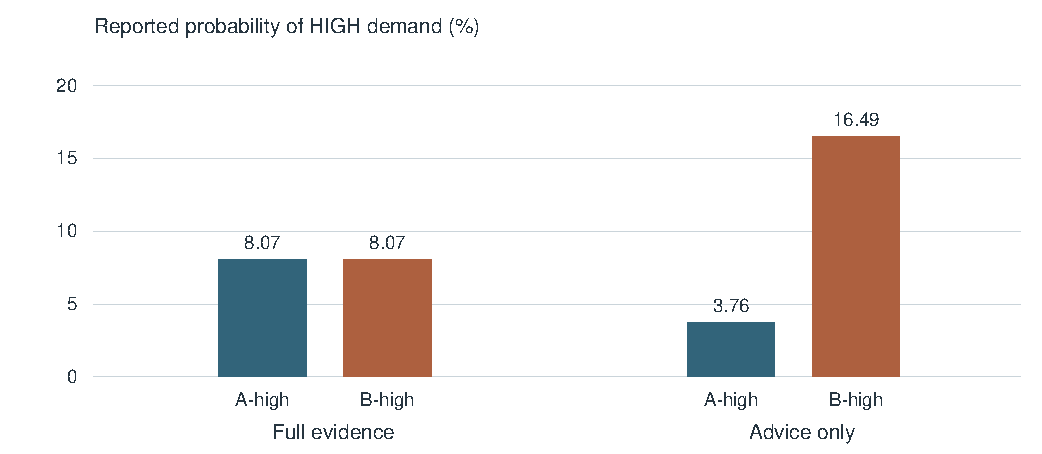
\includegraphics[width=.94\linewidth]{figures/case.pdf}
\caption{Agent 3 on the worked item. The horizontal labels identify the information condition and confidence assignment; the vertical axis is the reported probability of high demand in percent. Blue denotes A-high and brown denotes B-high. Each bar averages two calls; there are no error bars. This is one illustrative recorded item, not the batch estimate.}
\label{fig:case}\end{figure}

\subsection{Why the full-evidence response is near 8.07\%}
All 18 surveys contain six high and twelve low signals. The likelihood ratio for high versus low demand is
\begin{equation}
\frac{0.6^6\,0.4^{12}}{0.4^6\,0.6^{12}}=(2/3)^6=64/729.
\end{equation}
With equal priors, the full-evidence reference probability is therefore $64/(64+729)=64/793\simeq0.08070618$. Exchanging confidence labels does not change this reference. Agent 3's full-evidence outputs are close to it in both assignments.

The actual demand is low, but the evidence-based probability of high demand is not zero. Forecast quality against the realized state and agreement with the evidence-based reference are different evaluations.

\subsection{From one recipient to one item}
Agent 2 was also tested. Under advice only, its A-high outputs were 3.7553\% and 1.7037\%, averaging 2.7295\%. Both B-high outputs were 16.49484536\%. Its mean shift was 13.76534536 percentage points. The item-level shift is
\begin{equation}
\frac{12.73952536+13.76534536}{2}=13.25243536\text{ percentage points}.
\end{equation}
Thus 12.74 for one recipient, 13.25 for this item, and 22.48 for the replication batch describe different levels of averaging. They are not competing estimates of the same single response.

\takeaway{A score allocation can change a continuous forecast without flipping a binary answer. The worked example also shows genuine same-input variability in another recipient, which must be retained rather than selected away.}

\section{Batch results and their interpretation}
\label{sec:results}
\subsection{What was held fixed in replication}
The discovery batch generated 16 markets; all had valid mixed initial choices and entered updates. Its 96 initial and 512 update calls were all valid. The replication generated 16 new markets with the same prior and survey process. Fifteen had mixed initial choices; one unanimous item was excluded without replacement. Its 96 initial and 480 update calls were all valid.

The replication plan retained the model ID, prompts, score values, two recipients, information conditions, repeated-call count, and analysis. The task-generation seed changed from 20260919 to the prespecified 20260920. Allocation, execution-order, and bootstrap seeds remained 20260919. The date-like directory labels should not be read as the chronological execution dates.

No exact survey array recurred across batches, and no ordered vector of member-level high-signal counts recurred. Four replication items were nevertheless equivalent to old items when member identities were ignored and only the multiset of counts was retained. Replication therefore concerns new samples of the \emph{same mechanism}, not new task families.

\subsection{Definition of the primary measures}
Let $p_{qivr}^{B+}$ and $p_{qivr}^{A+}$ denote the reported high-demand probabilities for item $q$, recipient $i$, information condition $v$, and repetition $r$, under B-high and A-high. For each item,
\begin{equation}
\Delta_{qv}=\frac14\sum_{i=1}^{2}\sum_{r=1}^{2}
\bigl(p_{qivr}^{B+}-p_{qivr}^{A+}\bigr),\qquad
\Delta_v=\frac1Q\sum_{q=1}^{Q}\Delta_{qv}.
\end{equation}
The two recipients need not have IDs 1 and 2; the summation indexes the two selected recipients. Positive $\Delta_v$ means that moving the high score toward B shifts forecasts toward B. Multiplying by 100 expresses the difference in percentage points (pp). The main visibility comparison is
\begin{equation}
I=\Delta_{\mathrm{advice}}-\Delta_{\mathrm{full}}.
\end{equation}
A positive $I$ means a larger allocation effect when peer evidence is unavailable. This is a difference of score effects, not simply the difference between full and advice-only forecast levels.

All primary cells must be complete on a common item set. Each item receives equal weight. We obtain descriptive 95\% intervals by resampling items within actual high/low-demand strata 2,000 times, preserving all paired responses and each stratum's eligible size, and using the 50th and 1,950th sorted estimates. Individual calls are not treated as independent items.

\begin{table}[H]\centering\small
\begin{tabularx}{\linewidth}{@{}p{.28\linewidth}YY@{}}\toprule
Measure (pp) & Discovery: 16 items & Replication: 15 items \\\midrule
Full-evidence shift & $-0.06715$\newline $[-0.20231,\;0.00092]$ & $+0.000176$\newline $[0.000021,\;0.000441]$ \\
Advice-only shift & $+14.81$\newline $[10.34,\;19.65]$ & $+22.48$\newline $[17.38,\;27.90]$ \\
Advice minus full & $+14.87$\newline $[10.30,\;19.59]$ & $+22.48$\newline $[17.46,\;27.27]$ \\\bottomrule
\end{tabularx}
\caption{Mean score-allocation effects and descriptive item-bootstrap 95\% intervals. Each item first averages two recipients and two calls per input. The primary visibility interaction is positive in both batches. The very small positive full-evidence interval in replication does not imply a practically substantial effect.}
\label{tab:main}\end{table}

\begin{figure}[H]\centering
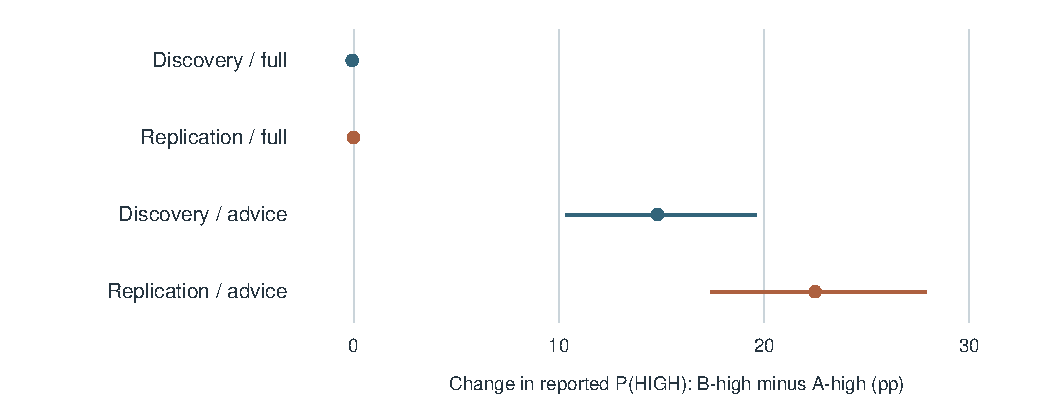
\includegraphics[width=\linewidth]{figures/results.pdf}
\caption{Batch-level score-allocation effects. The horizontal axis is B-high minus A-high in the reported probability of high demand, in percentage points. Rows separate batch and information condition; blue is discovery and brown is replication. Points are equal-item means, with descriptive 95\% item-bootstrap intervals. The full-evidence intervals are too small to resolve on this scale. There are 16 and 15 eligible items, not hundreds of independent tasks.}
\label{fig:results}\end{figure}

Advice-only shifts were positive on 15/16 discovery items and 15/15 replication items. The direction repeated, but the two batch magnitudes differ. The corresponding increases in the frequency of choosing B were 10.94 and 30.00 pp under advice only, and zero under full evidence. An unchanged option on the worked item is therefore compatible with option changes elsewhere.

\subsection{Does the shift improve the forecast?}
That requires a different outcome. For actual demand $y_q\in\{0,1\}$, with 1 meaning high, the Brier score is the average of $(\pB-y_q)^2$; smaller is better. The mean square deviation from the full-evidence probability is another measure. In advice only, the latter includes missing information and cannot be wholly attributed to faulty reasoning.

In the discovery batch the A-high advice condition had the better realized-state Brier score; in replication B-high had the better score. The intervention is tied to A/B stance, not truth. A directional forecast shift therefore does not establish a consistent benefit or harm. The current batches also provide no estimate of the final consensus effect in demand tasks.

\subsection{Does the result reveal a trust mechanism?}
The observed object is a response to a displayed number. In the worked example, the model's text interpreted different confidence assignments as different implied survey counts: approximately five high versus seven high, although the real count was six. A possible explanation is that displayed confidence is used as a cue to unobserved evidence strength. This remains an interpretation; generated reasons need not faithfully reveal internal computation.

A post-hoc explanatory calculation treated each displayed score as if it were a calibrated private probability, multiplying the recipient's private odds by $c/(1-c)$ for a B recommendation and $(1-c)/c$ for A. It predicted a discovery advice effect of about 16.34 pp, compared with 14.81 pp observed. This calculation was introduced after the first completed discovery item. It was not promoted to the replication's primary test. Because the host overwrote scores, its calibration premise is not guaranteed by the experiment.

\takeaway{The supported finding is a replicated local response to confidence allocation under missing peer evidence, with a much smaller mean response when all surveys are available. Internal trust, irrationality, harmful consensus, and predictive group dynamics remain unestablished.}

\section{Relation to previous work}
Confidence in multi-agent communication is already an established topic. ReConcile exchanges answers, explanations, and confidence and uses confidence-weighted voting~\cite{reconcile}. ConfMAD studies explicit confidence expression during debate~\cite{confmad}. Our local comparison keeps the opinions fixed and exchanges scores; the later group plan keeps the final aggregation rule fixed.

HiddenBench studies collective reasoning with distributed information~\cite{hiddenbench}. It motivates distinguishing private observations from information pooled across members. Our survey task is newly constructed, rather than a reproduction of that benchmark. KAIROS studies historical interactions and current peer responses under different peer reliability conditions~\cite{kairos}; our displayed current-answer score should not be confused with a sender's measured historical accuracy. Work on changes of mind further motivates controlling the visible initial answer~\cite{change}.

The longer-term aim is related to compact predictors of agent communities~\cite{physics} and analyses of biased consensus~\cite{biased}. The intended contribution is the combination of a content-controlled allocation intervention, an evidence-visibility comparison, and prospective local-to-group prediction. Neither ``confidence matters'' nor ``agents influence one another'' is claimed as novel by itself. The brief positioning here is not a claim of exhaustive novelty.

\takeaway{Prior work motivates the components. The additional evidence this project still needs is that a locally measured allocation response helps predict new group outcomes.}

\section{What remains to be done}
\label{sec:future}
The following are planned tests, not completed demand results. The present pilots informed task selection; they must not be relabeled as unseen confirmatory test data.

\subsection{First predict a new recipient response}
A small statistical predictor should first estimate the recipient's \emph{reported probability}, because that is the current primary outcome. A separate predictor can estimate the probability that a repeated response chooses B. These are different: the former concerns the model's forecast about demand, whereas the latter concerns the distribution of model outputs.

Compare a confidence-blind predictor, which knows the task information, the recipient's previous forecast, and peer recommendations, with a predictor that additionally knows score allocation. Full-evidence inputs must be available to both predictors in that condition. Candidate features can summarize the recipient's surveys, peer A/B counts, and score--stance association. For example, the sum of scores on B recommendations minus the sum on A recommendations is a transparent feature, not an assumed law of updating.

Use disjoint training, validation, and test items. Keep numerical variants, paraphrases, and option reversals in the same split. Fit on training items, choose settings on validation items, and then freeze the method. Evaluate reported-probability predictions by held-out squared error and binary-choice predictions by proper probability scores. Improvement must be measured over the best confidence-blind comparator on the same test items. A nonzero fitted coefficient or better training fit is insufficient.

\subsection{Then test a genuinely interacting group}
Extend the first update to all six agents. All read the same previous snapshot; completion order must not change their inboxes. The two selected senders do not see their own confidence field, so the full six-agent policy contrast need not preserve each recipient's score multiset. Continue reporting the strict unaffected-recipient local contrast separately from the whole-group allocation effect.

For subsequent updates, state exactly which fields are routed: original private surveys, latest own answer and probability if retained, and permitted peer messages. Begin with a bounded answer-sharing protocol; introduce generated reasons as a separate richer protocol. If a continuous own probability or a reason is retained, six binary answers alone are not a sufficient description of the next input. We therefore do not carry over the original proposal's unvalidated 64-answer-state approximation as an established model.

\begin{figure}[htbp]\centering
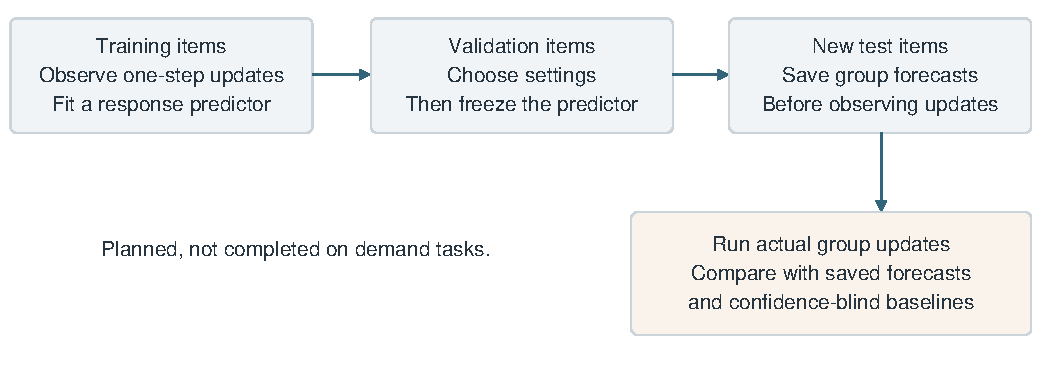
\includegraphics[width=\linewidth]{figures/prediction.pdf}
\caption{Planned local-to-group prediction test. Arrows indicate the research sequence, not experimental results. Test forecasts are saved before observing actual group updates. Predictors must not use future responses or newly observed future reasons during a free trajectory forecast. There are no numerical axes or uncertainty bars.}
\label{fig:prediction}\end{figure}

Before running a test group's continuation, save predictions of its future trajectory and final outcomes. During prediction, propagate predicted states rather than substituting the actual next response. Predicting group vote distributions may require a model of response variability, not only each agent's mean forecast: thresholding a mean at 0.5 does not determine how often individual responses exceed 0.5. These approximations need validation before interpreting a group forecast.

Keep unweighted aggregation fixed. With six agents, at least four votes establish a majority; a 3--3 split is a tie. Measure accuracy or forecast quality separately from agreement. Prespecify rounds and the main evaluation time before seeing continuation outcomes.

\subsection{Finally remove the displayed scores}
To study persistence, show the allocation intervention only in the first update. Within each allocation branch, copy the resulting state into two continuations: continued peer exchange and independent self-review. Both retain the task and use the same number of updates. Subsequent prompts omit the original score overlay and round-zero transcript. Continued discussion includes the latest permitted peer messages; self-review includes only the latest own state.

This asks whether the original effect remains and whether continued interaction changes it relative to self-review. If agents regenerate confidence wording themselves, record that event. Accidental retention of the old source text is a routing error. Different messages generated \emph{after} the intervention can legitimately transmit the effect.

An optional later test exposes just one recipient to a fixed source with high versus low confidence, keeps that source out of the final vote, and measures effects on the other five members who never see it directly. Only that restricted exposure design addresses indirect dissemination rather than shared direct exposure.

\subsection{Decisions based on evidence}
The next study size and spending cap should be set from item-level variability and a meaningful precision target, before test outcomes. Repeating one item more often cannot replace independent items. Cross-model and communication-graph extensions come after this first local-to-group validation. Null or poorly predicted effects remain valid outcomes.

\takeaway{The next claim to earn is out-of-sample predictive value. The larger goal is not completed by finding a larger local shift or by fitting a convenient equation after seeing the trajectories.}

\section{Implementation and current conclusion}
The saved demand requests use \texttt{openai/gpt-5.6-luna}, medium reasoning, a maximum of 8192 output tokens, and a strict JSON schema. There is no additional temperature or API-seed override. Provider fallback is disabled and required parameters are enforced. Four items can execute concurrently; update conditions and repetitions are randomized within an item. All branches share their saved initial state and settings. No GLM or Qwen comparison has yet been completed in this evidence set.

Raw input comparisons verify which fields change. The logs also allow checks for hidden-state leakage, invalid responses, truncated outputs, choice/probability inconsistency, usage, and repeated-input variability. Missing responses are not replaced with old answers or retried to obtain a preferred direction. Both demand batches returned valid responses for every scheduled call. Their recorded costs were approximately \$0.527820 and \$0.467750; these are historical response-usage totals, not current price quotes.

The present conclusion is limited but concrete: for one model and one controlled forecasting mechanism, assigning the higher displayed confidence to a different recommendation changes one-step reported probabilities much more when peer evidence is hidden. The direction recurs in new instances. We have not demonstrated that this behavior is irrational, worsens realized predictions consistently, or predicts a group's eventual judgment. Those distinctions organize the revised research plan.

\appendix
\section{How the task was selected: earlier experiments}
\label{app:history}
The two earlier task-search stages are kept here so that the main text can start with the final demand task. They are relevant negative and diagnostic evidence, not independent replications of the demand result.

\subsection{Stage 1: logical entailment and difficulty calibration}
The task asked whether Boolean premises necessarily imply a target proposition. A minimal natural-language example is: ``All students have a card; Wang is a student; must Wang have a card?'' The experimental L2 version used seven Boolean variables and 28 premises. Enumerating all $2^7=128$ assignments gives a verifiable answer: one satisfying assignment that falsifies the target suffices to refute entailment. Premises were jointly satisfiable.

The first two-task smoke run produced all-correct initial answers. A broader calibration used 24 items across three task families and four levels, with six calls each: 139/144 were valid and 130 valid responses were correct. Logic L1 and L2 initially had 7/12 and 9/12 correct responses, respectively. A four-item follow-up gave L1 12/12 and L2 10/12. On 20 new L2 items, 114/120 responses were correct; only three items had initial disagreement, and 17/20 correct labels were non-entailment.

A balanced bank then used 40 items: 20 entailment and 20 non-entailment, with A/B correct-option labels balanced within each class. Candidate filtering used the verifier, not observed model performance. Of 240 calls, 230 were valid and 186 were correct (80.9\%). Fifteen items had complete mixed-correctness responses. Eight outputs were truncated at the old 2048-token cap and two had format errors. All 44 wrong valid responses reported chosen-answer confidence at least 0.99, with mean about 0.996.

For a recorded disagreement example, expansion item v4 asked whether $X_1$ necessarily follows. Six assignments satisfied its premises; one was $(0,0,1,0,1,0,1)$, so entailment failed. The six responses were A,A,A,B,A,A; the fourth was wrong and reported 99\% confidence. This illustrates verification, not post-hoc selection for the later main bank.

An output-reliability test revisited all eight previously truncated items, six calls each. Changing the output cap to 8192, reasoning to medium, and response format to strict JSON yielded 48/48 valid responses. Because all three settings changed together, their individual contributions cannot be identified. The maximum new output was 1897 tokens, so this test alone does not show that a larger cap caused the improvement.

\paragraph{Fixed-opinion score experiments.}
The next tests supplied scripted previous answers and four scripted peers rather than real six-agent initial responses. Each peer panel had two correct and two incorrect opinions. The four conditions assigned 0.95/0.55 to the correct/incorrect camps, reversed that assignment, gave everyone 0.75, or hid scores. On 40 items with three calls per condition, 479/480 responses were valid or observable; one remained pending. The complete-item contrast was the error rate under incorrect-high minus correct-high: $-1.71$ pp over 39 items, with interval $[-8.55,5.13]$. Eight item effects were positive, eight negative, and 23 zero.

An eight-condition experiment varied the score gap using 0.80/0.70, 0.90/0.60, and 0.95/0.55, each in both directions, plus equal and hidden conditions. Each cell had three calls. On the reused 40 items, 954/960 were valid. Fitting an item-wise linear slope across gaps 0.10, 0.30, and 0.40, then averaging 36 complete items, gave $-4.63$ pp in the error contrast per 0.10 increase in gap, with interval $[-8.00,-1.46]$. The direction was contrary to the motivating expectation. Label audits did not find reversed treatment coding.

On 40 new balanced items under the same eight-condition protocol, 952/960 responses were valid. The complete-item slope was $-0.26$ pp per 0.10 gap, with interval $[-4.23,3.57]$, over 36 items. The negative trend did not clearly replicate. The earlier four-condition and eight-condition runs also had different confidence-definition instructions, so they should not be pooled without a protocol distinction. Post-hoc diagnostics across 80 items found item-class and within-input variation but did not establish the cause of the initial reverse trend.

\takeaway{Logic provided verifiable answers and exposed sampling and formatting issues. It did not provide a stable direction of confidence-induced error. Scripted initial opinions and the ability to solve the full task independently motivated a task with genuine distributed information.}

\subsection{Stage 2: supplier choice with distributed records}
Agents selected the supplier with the greater total net benefit. One audit record was public; six others were private, one per agent. Initially unseen A-minus-B contributions were assigned expected value zero under the stated prior. Each agent first answered using its available records. On updates all records were disclosed.

\begin{table}[htbp]\centering\small
\begin{tabular}{@{}lrrr@{}}\toprule
Record (training item 00) & Supplier A & Supplier B & A minus B \\\midrule
Public &27&31&$-4$\\
Private to agent 0&60&71&$-11$\\
Private to agent 1&71&64&$+7$\\
Private to agent 2&60&61&$-1$\\
Private to agent 3&69&67&$+2$\\
Private to agent 4&46&44&$+2$\\
Private to agent 5&44&36&$+8$\\\midrule
Total&377&374&$+3$\\\bottomrule
\end{tabular}
\caption{A real supplier item. Agent 0 initially sees an A-minus-B total of $-15$ and chooses B; agent 1 sees $+3$ and chooses A. Once all records are visible, supplier A has the larger total. Private-information choices need not match this full-information answer.}
\end{table}

The six initial responses in this item were B,A,B,B,B,A. Across eight training and eight test items, all roots had disagreement. There were 112 initial/full-information-control calls, 192 local updates, and 288 group updates, all valid, for 592 total. Scores 0.95 and 0.55 were exchanged between one initially correct and one incorrect sender; other members had 0.75. Strict local comparisons used the other four receivers.

With all records available, the strict training recipients were correct under both main allocations. Test groups were all correct in the first update under the three group conditions. In the second update, errors numbered 0/48, 2/48, and 1/48 for aligned, misaligned, and hidden-score branches. However, for every matched item and member, the three second-update request hashes were identical. Scores and the original history were absent, while the first-update choices had converged. Those few errors are therefore not evidence of propagated treatment differences.

A logistic predictor was fitted on training items and frozen before test continuations. Compared with a confidence-blind version, adding scores did not improve prediction: first-round behavioral Brier scores were 0.046554 versus 0.046153, and second-round scores were 0.043829 versus 0.042062 (smaller is better). It used eight training and eight test items; the fact that this pipeline ran does not demonstrate useful local-to-group prediction.

\takeaway{Genuine private-information initial responses were feasible. Full evidence made this additive task almost uniformly easy, leaving little treatment effect to predict. The demand task was introduced to compare evidence visibility directly within one controlled setting.}

\section{Complete run inventory and analysis qualifications}
\label{app:inventory}
Table~\ref{tab:inventory} accounts for all twelve completed real runs in the report. Their calls are not independent task counts: several runs reuse the same items. Directory suffixes identify runs or seeds, rather than a reliable execution chronology.
\begin{table}[htbp]\centering\small
\begin{tabularx}{\linewidth}{@{}lp{.32\linewidth}rY@{}}\toprule
ID & Purpose & Valid / calls & Main sample or outcome \\\midrule
E01 & Workflow smoke test &124/124&Two tasks; all initial answers correct.\\
E02 & Three-family calibration &139/144&24 tasks; logic L1/L2 selected for follow-up.\\
E03 & L1/L2 follow-up &24/24&Four new tasks.\\
E04 & L2 expansion &120/120&20 tasks; three had disagreement.\\
E05 & Balanced L2 calibration &230/240&40 tasks; 186 correct valid responses.\\
E06 & Output-reliability retest &48/48&Eight previously failed tasks.\\
E07 & Four-condition local test &479/480&Scripted opinions; main interval crossed zero.\\
E08 & Score-gap exploration &954/960&Reused 40 tasks; negative slope.\\
E09 & Score-gap replication &952/960&40 new tasks; negative slope not established.\\
E10 & Supplier local/group test &592/592&8 training and 8 test items; no predictive gain.\\
E11 & Demand discovery &608/608&16 eligible markets.\\
E12 & Demand replication &576/576&15 eligible of 16 planned markets.\\\bottomrule
\end{tabularx}
\caption{Completed real runs, including invalid or unresolved requests in denominators. Two failed account-start attempts and six mock-run directories are excluded from this evidence inventory.}
\label{tab:inventory}\end{table}

There are 4,876 request records and 4,846 valid responses. Recorded costs sum to \$4.826184, with 15 request costs unknown. Of 4,861 responses with prompt-cache metadata, none reported cached input tokens; 15 lacked that metadata. Reusing a saved initial state across treatments is distinct from provider prompt-cache billing. Repeated response samples must not be replaced by a cached answer.

\paragraph{Missingness.}
The logic runs retained failures rather than resampling for desired answers. Primary summaries used complete item sets. Separately assigning all missing outcomes their best/worst values gives missing-data ranges, not sampling confidence intervals. In the new score-gap run, the full-40-item slope range was $+0.89$ to $+1.31$ pp per 0.10 gap, unlike the complete-36-item estimate of $-0.26$. These concern different item populations; neither should silently replace the other.

\paragraph{Scope of auxiliary checks.}
Offline diagnostics of the 80 logic items added no model calls. Demand checks also examined repeat variability, per-item direction, initial majority-rule agreement, schema validity, and paired input differences. In both demand batches all 96 initial choices followed the private-survey majority rule. That supports the interpretation of the initial states in these batches, but it does not establish a universal update rule after social information arrives.

\paragraph{Precision and generalization.}
The demand bootstrap describes uncertainty across the sampled markets under one generator. It does not quantify variation across model families or task mechanisms. A narrow interval around a tiny full-evidence effect is not a practically meaningful effect merely because it excludes zero. Conversely, a wide interval crossing zero does not prove invariance. Predefining an equivalence margin would be needed for a stronger negligible-effect claim.

\paragraph{Source mapping.}
The two main data directories are
\begin{quote}\small\ttfamily
runs/signal-visibility-luna-20260919\\
runs/signal-visibility-replication-20260920
\end{quote}
Their \texttt{manifest.json}, \texttt{roots.json}, \texttt{updates.json}, and \texttt{summary.json} contain settings, saved initial states, responses, and summaries. \texttt{PROTOCOL.md} records the design; the replication additionally has \texttt{REPLICATION\_PLAN.md}. Individual requests reside under each item's \texttt{calls} directory. Prompt examples shipped with these notes retain their source paths. Earlier runs are described in the accompanying full local report; no new model calls were made to write these notes.

\section{Literal prompt examples and reproduction details}
\label{app:prompts}
The examples below come from replication item \texttt{demand-00}, agent 3. JSON formatting is adjusted for readability; keys, values, and array order are retained. The accompanying \texttt{prompt\_examples.json} includes five complete original request objects and their parsed outputs. Within each condition, we use the first matching saved call in filename order as an example; batch statistics use all scheduled outputs.

\subsection{Complete initial user message}
The common system message is printed in Section~\ref{sec:prompts}. This is the entire initial user payload:
\lstinputlisting[basicstyle=\footnotesize\ttfamily]{prompts/initial_formatted.json}
The \texttt{meaning} field explains conditional independence and single counting. The \texttt{source\_id} fields identify observations uniquely. There is no true-state field.

\subsection{Complete advice-only, A-high user message}
This update uses the identical system message and adds genuine previous-answer and peer-report fields:
\lstinputlisting[basicstyle=\footnotesize\ttfamily]{prompts/advice_A_high_formatted.json}
For B-high, replace only the selected agent-4 and agent-1 confidence values as shown in Table~\ref{tab:swap}. For full evidence, add each peer's original three surveys, using Table~\ref{tab:initial}; Section~\ref{sec:prompts} gives one complete expanded peer entry. Both complete full-evidence requests are in the accompanying JSON. The host asserts that swapping the two scores transforms each A-high payload into its B-high counterpart, and removing peer survey arrays transforms full evidence into advice only.

\clearpage
\subsection{API settings are not part of the task answer}
Every example uses the same model, output cap, reasoning effort, provider settings, and schema. The request configuration is:
\lstinputlisting[basicstyle=\footnotesize\ttfamily]{prompts/request_configuration.json}
No extra temperature or API seed is supplied in these request objects. Initial reasons are saved but not forwarded to peers. The strict schema helps separate invalid output from an incorrect substantive answer; it does not force the reported probability to equal the mathematical reference.

\section{Revision from the original proposal}
This version preserves the central sequence: controlled local intervention, new-item replication, prospective group prediction, and removal of the original cue. It replaces assumptions that are not supported by the current task or evidence:
\begin{itemize}
\item Current-score allocation is defined by A/B stance. Correctness, realized-state forecast quality, and full-evidence probability are evaluated separately.
\item Reported probability is a primary behavior; an answer-only transition model would miss demonstrated changes below the choice threshold.
\item Unverified parametric influence weights, contraction claims, and answer-only state sufficiency are not premises of the revised empirical argument. Removing them is not a claim that their conditional mathematical statements were false.
\item The old 160-item division and approximately 30,000-call scenario are not commitments. The next design needs a precision target and a measured budget.
\item Multiple graphs, backbones, and task families are extensions after the first controlled local-to-group test, rather than simultaneous main-study requirements.
\end{itemize}
The original source remains in the repository for provenance. Its full text is not appended to these revised notes. Earlier null or unreplicated experiments remain in Appendix~\ref{app:history}, because revising a proposal must not remove inconvenient observations.

\begin{thebibliography}{9}
\bibitem{reconcile} J. C.-Y. Chen, S. Saha, and M. Bansal.
\emph{ReConcile: Round-Table Conference Improves Reasoning via Consensus among Diverse LLMs}. ACL 2024 version.
\url{https://arxiv.org/abs/2309.13007v3}.
\bibitem{confmad} Z. Lin and B. Hooi.
\emph{Enhancing Multi-Agent Debate System Performance via Confidence Expression}. Findings of EMNLP, 2025.
\url{https://aclanthology.org/2025.findings-emnlp.343/}.
\bibitem{hiddenbench} Y. Li, A. Naito, and H. Shirado.
\emph{Systematic Failures in Collective Reasoning under Distributed Information in Multi-Agent LLMs}. Version 4, 2026.
\url{https://arxiv.org/abs/2505.11556v4}.
\bibitem{kairos} M. Song et al.
\emph{LLMs Can't Handle Peer Pressure: Crumbling under Multi-Agent Social Interactions}. Version 1, 2025.
\url{https://arxiv.org/abs/2508.18321v1}.
\bibitem{change} D. Kumaran et al.
\emph{How Overconfidence in Initial Choices and Underconfidence Under Criticism Modulate Change of Mind in Large Language Models}. 2025.
\url{https://arxiv.org/abs/2507.03120v1}.
\bibitem{physics} B. El et al.
\emph{Physics of Agents: Statistical Mechanics Predicts Collective Behavior of AI Agents}. Version 2, 2026.
\url{https://arxiv.org/abs/2608.16578v2}.
\bibitem{biased} M. Okawa.
\emph{Emergence of Biased Consensus in Multi-Agent LLM Debates}. Version 1, 2026.
\url{https://arxiv.org/abs/2608.02827v1}.
\end{thebibliography}
\end{document}
